\chapter{Experiment na $2$-hranovo súvislých grafoch}

V prvej kapitole sme sa venovali konštrukcii algoritmu, ktorý dokáže z efektívneho riešenia
problému $L(2,1)$-farbenia na chlpatých $2$-hranovo-súvislých grafoch vyskladať efektívne
riešenie problému $L(2,1)$-farbenia na všeobecných grafoch.

Najefektívnejšie riešenie problému $L(2,1)$-farbenia má časovú zložitosť zhora ohraničenú
počtom vlastných párov na súvislých grafoch. Pripomenieme, že vlastný pár grafu $G$ je
dvojica $(S, X)$ podmnožín vrcholov grafu $G$, kde $S$ je $2$-pakovanie a $S \cap X = \emptyset$.
V tejto kapitole sa budeme venovať experimentálnemu odhadu počtu vlastných párov na
$2$-hranovo súvislých grafoch.

Cieľom experimentu bolo odhaliť, aký typ $2$-hranovo súvislých grafov má najviac
vlastných párov.

\section{Konštrukcia $2$-hranovo súvislých grafov}

Najprv popíšeme a dokážeme spôsob, ktorým vieme skonštruovať všetky $2$-hranovo
súvislé grafy. Bude sa nápadne ponášať na konštrukciu $2$-súvislých grafov. Každý
$2$-hranovo súvislý graf sa dá vytvoriť z kružnice pridávaním $H$-ciest do existujúceho
grafu \cite{diestel_graph}. Tento postup vieme rozšíriť na $2$-hranovo súvislé grafy, ak
dovolíme okrem $H$-ciest pridávať aj $H$-kružnice.

\begin{defn}
    Nech $H$ je graf. Cestu $P$ budeme nazývať $H$-cesta, ak prienik $P$ a $H$ tvoria
    práve koncové vrcholy $P$.

    Kružnicu $C$ budeme nazývať $H$-kružnica, ak prienik $C$ a $H$ tvorí
    práve jeden vrchol.
\end{defn}

\begin{veta}
    Každý $2$-hranovo súvislý graf $G$ sa dá vytvoriť z kružnice postupným pridávaním
    $H$-ciest a $H$-kružníc do grafov $H$, ktoré sme už skonštruovali.
\end{veta}
\begin{proof}
    Najprv dokážeme, že $G$ obsahuje kružnicu ako podgraf. Graf $G$ je $2$-hranovo súvislý,
    preto pre ľubovoľnú hranu $(uv) = e \in E(G)$ platí, že graf $G - e$ je súvislý. Nájdeme
    cestu $P$ medzi vrcholmi $u$ a $v$ v grafe $G - E$. Cesta $P$ doplnená o hranu $e$ tvorí
    kružnicu.

    Ďalej budeme postupovať sporom, graf $G$ sa nedá zostrojiť popísaným spôsobom. Graf $G$
    obsahuje kružnicu a teda existuje nejaký podgraf $G$, ktorý sa dá týmto spôsobom
    skonštruovať. Označme $H$ ako najväčší (vzhľadom na inklúziu) takýto podgraf.

    Ak by existovala hrana $(uv) \in E(G) - E(H)$, ktorej koncové vrcholy $u, v$ ležia v
    $H$, tak $(uv)$ tvorí $H$-cestu a teda je v spore s maximálnosťou $H$. To znamená, že
    $H$ je indukovaný podgraf.
    
    Graf $G$ je súvislý a teda v ňom musí existovať hrana
    medzi nejakou dvojicou vrcholov $u, v$, kde $u \in V(G) - V(H)$ a $v \in V(H)$.
    Z predpokladu, že $G$ je $2$-hranovo súvislý vieme, že $G - (uv)$ je súvislý a teda
    v ňom existuje nejaká cesta $P$ medzi vrcholom $u$ a $v$. Nech $w$ je posledný vrchol
    na ceste $P$ z množiny $V(G) - V(H)$ a $P_w$ je časť cesty $P$ od vrchola $w$ do $v$.
    Cesta $P_w$ s hranou $(uv)$ tvorí $H$-cestu, ak $w \neq u$, alebo $H$-kružnicu, ak $w = u$.

    To znamená, že pridaním cesty $P_w$ s hranou $(uv)$ do grafu $H$ dostaneme väčší graf,
    ktorý vieme skonštruovať popísaným postupom. To je však v spore s predpokladom, že $H$ je
    maximálny podgraf, ktorý vieme týmto postupom skonštruovať.
\end{proof}

Za zmienku stojí fakt, že dôkaz vety nám dáva spôsob, ako pre ľubovoľný graf určiť
postupnosť operácií, ktorými ho vieme vytvoriť.

Množinu všetkých $2$-hranovo súvislých grafov s daným počtom vrcholov teda vieme skonštruovať
nasledovne: Najprv určíme, aký veľký je prvý cyklus a pre každú túto možnosť spustíme
rekurzívnu procedúru, ktorá pridáva $H$-kružnice a $H$-cesty.

Rekurzívna procedúra dostane ako parameter nejaký $2$-hranovo súvislý graf $H$ a počet
vrcholov $k$, ktoré treba ešte do grafu pridať.

Pridávanie $H$-ciest bude fungovať nasledovne: Pre každý možný výber dvojice rôznych
vrcholov $u, v$ a každú možnosť počtu nových vrcholov $p \leq k$ vytvorí graf $H'$,
Graf $H'$ vznikne z grafu $H$ pridaním cesty s $p$ novými vrcholmi medzi vrcholy $u, v$.
Nakoniec rekurzívne spustí túto procedúru s parametrami $H'$ a $k - p$.

Pridávanie $H$-cyklov bude fungovať podobne: Pre každý vrchol $v$ a pre každý možný
počet nových vrcholov $2 \leq p \leq k$ skonštruujeme graf $H'$. Graf $H'$ vznikne z
grafu $H'$ pridaním cyklu s $p+1$ vrcholmi, kde jeden z nich je $v$. Na graf $H'$
rekurzívne spustíme procedúru s parametrami $H'$ a $k - p$.

Takto popísaný algoritmus pre konštrukciu $2$-hranovo súvislých grafov je nepraktický,
lebo väčšinu $2$-hranovo súvislých grafov vieme podľa predošlého postupu skonštruovať
viackrát. Pri skúmaní počtu vlastných párov nás nezaujíma označenie vrcholov. Preto stačí,
ak každý neoznačený $2$-hranovo súvislý graf skonštruujeme aspoň raz.

V ďalšej časti si popíšeme viacero spôsobov, ktorými vieme zredukovať množstvo vygenerovaných
grafov. Postupne tak načrtneme základný algoritmus a $5$ zlepšení, ktoré nakoniec medzi
sebou porovnáme.

\section{Redukcia počtu grafov}

Pripomeňme si viackrát využitý fakt: odobratím ľubovoľnej hrany z grafu sa jeho počet vlastných
párov nezníži. Ak nás teda zaujímajú grafy s najväčším počtom vlastných párov, môžeme sa obmedziť
na také, ktoré nemajú hrany navyše. Z pohľadu nášho algoritmu na vytváranie $2$-hranovo súvislých
grafov to znamená, že stačí pridávať iba také $H$-cesty, ktoré obsahujú aspoň jeden nový vrchol.

Ďalší jednoduchý spôsob, ako vieme zmenšiť počet vygenerovaných grafov je nasledovný: $H$-cestu
medzi vrcholy $u, v$ pridáme iba vtedy, ak nejde o susedné vrcholy. Dôvod si zhrnieme v nasledujúcej
leme.

\begin{lema}
    Nech $H$ je $2$-hranovo súvislý graf, nech $u, v$ sú vrcholy v $H$ spojené hranou $e$.
    Nech graf $H'$ vznikne z $H$ pridaním cesty $P$ medzi vrcholy $u, v$. Potom $H' - e$ je
    $2$-hranovo súvislý graf.
\end{lema}
\begin{proof}
    Dokážeme, že pre ľubovoľnú hranu $f \in E(H - e)$ platí, že graf $H' - \{e, f\}$ je súvislý.
    Graf $H$ je $2$-hranovo súvislý, čiže $H - e$ je súvislý. Zároveň je $H - e$ podgrafom
    $H' - e$.
    
    Pokiaľ vezmeme hranu $f$ z cesty $P$, tvrdenie platí, lebo pre každý nový vrchol v $P$
    existujú dve hranovo disjunktné cesty do grafu $H - e$ a graf $H - e$ je súvislý. 
    
    Pre hrany v grafe $H - e$ použijeme Mengerovu vetu. Pre každú dvojicu vrcholov
    v $2$-hranovo súvislom grafe existujú dve hranovo disjunktné cesty \cite{diestel_graph}.

    Vezmime ľubovoľné dva vrcholy $u, v$ a dve hranovo disjunktné cesty $P_1, P_2$ medzi nimi.
    Nanajvýš jedna z ciest obsahuje hranu $e$.
    Ak žiadna z nich neobsahuje hranu $e$, tak $P_1$ a $P_2$ je dvojica hranovo disjunktných ciest
    medzi $u, v$. Ak jedna z nich hranu obsahuje, bez ujmy na všeobecnosti je to $P_1$, tak túto hranu
    nahradíme cestou $P$.

    Pre ľubovoľnú dvojicu vrcholov $u, v \in V(H)$ teda platí, že existuje dvojica hranovo disjunktných
    ciest medzi $u$ a $v$ v grafe $H' - e$. Ak pre súvislý graf platí, že $G - (xy)$ je nesúvislý, vrcholy
    $x$ a $y$ musia ležať v rôznych komponentoch súvislosti $G - (xy)$. Keďže ľubovoľná dvojica vrcholov
    vo $V(H)$ je spojená dvomi hranovo disjunktnými cestami v $H' - e$, hrana $(xy) \in E(H) - \{e\}$ patrí
    nanajvýš do jednej z týchto ciest. Vrcholy $x, y$ teda ležia v tom istom komponente súvislosti grafu
    $H' - \{e, (xy)\}$ a teda graf $H' - \{e, (xy)\}$ je súvislý.

    Nech zvolíme ľubovoľnú hranu $e' \in E(H' - e)$, graf $H' - \{e, e'\}$ je súvislý. Graf $H' - e$ teda
    spĺňa definíciu hranovej $2$-súvislosti.
\end{proof}

Obe tieto zlepšenia implementujeme už v základnom programe. Ďalej budeme redukovať symetrie na základe
najväčšieho cyklu.

\subsection{Najväčší cyklus v grafe}

Prvý spôsob odstraňovania symetrií sa bude týkať najväčšieho cyklu v grafe. Ľubovoľný $2$-hranovo
súvislý graf $G$ môžeme našim postupom vypestovať tak, že najväčší cyklus v $G$ bude zodpovedať
cyklu, ku ktorému pridávame $H$-cesty a $H$-kružnice. Našej funkcii teda pridáme číselný parameter
$c$, ktorý bude popisovať najväčší cyklus, ktorý sa môže nachádzať v pestovanom grafe.

Pri pridávaní $H$-cyklu môžeme pridať nanajvýš $c - 1$ nových vrcholov, ináč vyrobíme väčší
cyklus, ako $c$. Pri pridávaní $H$-cesty medzi vrcholy $u, v$ môžeme pridať iba $c - l(u,v) - 1$ nových
vrcholov, kde $l(u,v)$ označuje dĺžku ľubovoľnej cesty medzi $u, v$. Pri prvom zlepšení budeme
ako $l(u,v)$ používať vzdialenosť $d(u,v)$, lebo sa dá rýchlo počítať.

V každom behu rekurzívnej funkcie teda pre každu dvojicu už existujúcich vrcholov spočítame
ich vzdialenosť Floyd-Warshallovym algoritmom, ktorý na grafe s $n$ vrcholmi pracuje v čase
$O(n^3)$.

Ako poznámku pridáme, že v skutočnosti náš druhý algoritmus nebol tesný, lebo pri pridávaní $H$-cyklu
sme mohli pridať až $c$ vrcholov a pri pridaní $H$-cesty medzi vrcholy až $c - d(u,v)$ vrcholov.

\subsection{Minimálne $2$-hranovo súvislý graf}

V treťom algoritme naplno využijeme vlastnosť, že odstránenie hrany nezmenšuje počet vlastných
párov. Zaujímať nás budú teda také grafy $H$, v ktorých platí, že graf $H - e$ nie je $2$-hranovo
súvislý. Takéto grafy sa nazývajú \emph{minimálne $2$-hranovo súvislé}.

Ak niektorý $2$-hranoco súvislý podgraf $G \subseteq H$ nie je minimálne $2$-hranovo súvislý,
tak ani graf $H$ nemôže byť $2$-hranovo súvislý \cite{min2con}. Ak teda v ktoromkoľvek volaní
rekurzívnej funkcie dostaneme graf $H$, ktorý nie je minimálne $2$-súvislý, nemá zmysel s ním
naďalej pracovať.

Overovať, či je graf minimálne $2$-hranovo súvislý, budeme nasledovne: Pre každú hranu $e \in E(H)$
pomocou Tarjanovho algoritmu overíme, či graf $H - e$ obsahuje most. Ak pre niektorú hranu graf $H - e$
neobsahuje most, tak $H$ nie je $2$-hranovo súvislý. Časová zložitosť kontroly je $O(m^2)$.

Toto zlepšenie výrazne zredukovalo počet vytvorených grafov, ako uvidíme v tabuľke.

\subsection{Usporiadané pridávanie ciest a cyklov}

V ľubovoľnom postupe vytvárania $2$-hranovo súvislého grafu môžeme operácie pridávania $H$-ciest
a $H$-kružníc vhodne usporiadať. Využijeme, že v našej reprezentácii máme vrcholy očíslované
číslami $0 \ldots n-1$. Pridanie $H$-cesty medzi vrcholy s číslami $u, v$, kde $u > v$, vieme symbolicky
reprezentovať ako dvojicu čísel $(u,v)$. Podobne pridanie $H$-cyklu pripojeného k vrcholu s číslom $u$
môžeme reprezentovať ako dvojicu čísel $(u,u)$.

Pri ľubovoľnom postupe vytvárania grafu môžeme vymeniť dve operácie s reprezentáciami (v poradí)
$X = (x_1,x_2)$ a $Y = (y_1, y_2)$ vymeniť, ak je $Y$ lexikograficky menšia ako $X$. Ak pri
vykonávaní operácie $X$ graf obsahoval vrchol $x_1$, tak musel obsahovať aj menší (rovný) vrchol $y_1$
a menší (rovný) vrchol $y_2$.

Týmto sme zavŕšili popis štvrtého algoritmu.

FIXME: Dá sa dokázať, že každý označený graf vygenerujeme najviac raz?

\subsection{Najväčší cyklus v grafe znova}

Ďalšie zlepšenie sa bude opäť týkať najväčšieho cyklu. Pre vopred stanovené $c$ môžeme medzi vrcholy
pridať nanajvýš $c - l(u,v) - 1$ nových vrcholov, kde $l(u,v)$ označuje dĺžku nejakej cesty. Pri
tomto zlepšení budeme budeme $l(u,v)$ počítať ako dĺžku najdlhšej cesty medu $u$ a $v$.

Zisťovanie dĺžky najdlhšej cesty medzi dvomi vrcholmi je NP-ťažký problém. Popíšeme riešenie
v čase $O(n^32^n)$, ktoré používa dynamické programovanie. Pre každý z $n$ vrcholov spočítame
najdlhšiu cestu z neho do každého iného vrchola. Ďalej popíšeme, ako vyzerá hľadanie najdlhšej
cesty z vrchola $u$ do ostatných.

Podproblém bude vyzerať nasledovne: Pre daný vrchol $v$ a nejakú podmnožinu dovolených
vrcholov $S$, aká je najdlhšia cesta z $v$ do $u$, ak môžeme použiť iba vrcholy v $S$?

Pre $v = u$ je odpoveď $0$. Pre $v \neq u$ sa pozrieme na všetkých susedov $w$ vrcholu $v$,
ktorí sú v množine $S$. Pre každého z nich spočítame najdlhšiu cestu z vrcholu $w$ do vrcholu
$u$, ktorá môže použiť iba vrcholy v $S - \{v\}$. Nech najväčšiu hodnotu nadobúdal nejaký vrchol
$w_{max}$. Potom odpoveď pre $v, S$, je o jedna väčšia, ako odpoveď pre $w_{max}, S - \{v\}$.
Najdlhšia cesta z vrcholu $x$ do $u$ potom zodpovedá riešeniu problému $x, 2^{V(G)}$.

Stavov je $n2^n$, pre každý z nich vyskúšame $O(n)$ možností. Celé riešenie s dynamickým
programovaním budeme spúšťať $n$-krát. Preto je časová zložitosť $O(n^32^n)$.

Všetky doteraz popísané zlepšenia sme vedeli vypočítať v polynomiálnom čase od veľkosti grafu.
Toto zlepšenie má však exponenciálnu časovú zložitosť od počtu vrcholov. Ukázalo sa,
že ho nie je dobré aplikovať úplne v každom kroku výpočtu. Čas, ktorý strávime počítaním
najdlhšej cesty v grafe, preváži čas, ktorý ušetríme orezaním niektorých vetiev výpočtu.

Ukázalo sa však, že ak budeme hľadať najdlhšiu cestu pre všetky grafy $H$, ktoré potrebujú
doplniť aspoň $3$ nové vrcholy a pre zvyšné, veľké grafy, budeme používať najkratšie cesty,
celkovo ušetríme zhruba polovicu času. Tento empirický fakt je, pochopiteľne, závislý od
časovej náročnosti operácie, ktorú na grafoch vykonávame. Pre rôzne výpočty nad grafmi
teda môže byť výhodnejšie počítať najdlhšie cesty na menších, alebo aj väčších grafoch.

\subsection{Symetria prvého cyklu}

Posledné vylepšenie sa bude týkať úplne prvej kružnice. Prvé pridanie $H$-cesty alebo $H$-kružnice
sa musí vykonať na niektorom vrchole, resp. dvojici vrcholov z prvej kružnice.
Nech je postupnosť pridávania $H$-ciest a $H$-cyklov ľubovoľná, môžeme ju otočiť tak, aby jeden
z vrcholov kružnice, ku ktorej pridávame $H$-cestu alebo $H$-kružnicu,
bol vrchol s číslom $0$.

\section{Počítanie vlastných párov}

Na počítanie vlastných párov využijeme vzorec $pp(G) = \sum \limits_{\substack{S \in \mathcal{P}(V_G) \\ S \textrm{ je } 2 \textrm{-pakovanie}}} 2^{n - |S|}$.
Pre každé $x$ vypočítame počet $2$-pakovaní, ktoré majú presne $x$ vrcholov.

Najrv pre každý vrchol $v \in V(G)$ vypočítame zoznam vrcholov, ktoré sú od neho vzdialené
nanajvýš $2$. Tento zoznam pre vrchol $v$ označíme $N^2[v]$.
Ďalej budeme generovať všetky $2$-pakovania grafu $G$ rekurzívnou funkciou.

Naša rekurzívna funkcia bude mať dva parametre, číslo aktuálneho vrcholu $i$ a zoznam zakázaných
vrcholov $S$. Naša funkcia sa vždy rekurzívne zavolá s parametrami $i+1$ a $S$, čo zodpovedá
situácii, keď vrchol $i$ nepridáme do $2$-pakovania. Ak vrchol $i$ nie je v ozname $S$, tak
navyše rekurzívne spustíme funkciu s parametrom $i$ a $S \cup N^2[i]$.

Každé volanie rekurzívnej funkcie vedie k nejakému $2$-pakovaniu. Pozrime sa, koľko operácií sme
spravili pri postupnosti výpočtov, ktoré viedli k danému $2$-pakovaniu. V každom z presne $n$
rekurzívnych volaní sme vykonali buď $O(1)$ operácií, ak sme daný vrchol nevzali do $2$-pakovania,
alebo $O(n)$ operácií, ak sme daný vrchol zobrali do $2$-pakovania a pridávali jeho okolie do
zoznamu $S$. Časová zložitosť hľadania všetkých $2$-pakovaní grafu $G$ je teda $O(n^3 + n^2P(G))$,
kde $P(G)$ je počet $2$-pakovaní v grafe $G$.

\subsection{Vlastné páry na cestách a kružniciach}

Pre dostatočne jednoduché triedy grafov vieme počet vlastných párov v závislosti
od veľkosti grafu vyjadriť cez rekurentný vzťah. Najprv ukážeme, ako sa dá vypočítať počet
vlastných párov na ceste s $n$ vrcholmi a následne pomocou neho vyjadríme počet vlastných
párov na kružnici s $n$ vrcholmi. Z rekurentného vzťahu nakoniec odvodíme asymptotický odhad
pre počet vlastných párov na cestách a kružniciach.

Počet vlastných párov cesty s $n$ vrcholmi označíme $p_n$. Pre $n > 3$ vieme rekurentný
vzťah vyrobiť nasledovne: Pozrieme sa na koncový vrchol $v$ cesty $P$. Vlastné páry $(S,X)$ rozdelíme
na tie, v ktorých vrchol $v$ patrí do $2$-pakovania $S$ a tie, v ktorých nepatrí.

Všetky vlastné páry
prvého druhu majú nasledovný tvar: Sused $u$ vrchola $v$ ani sused $w$ vrchola $u$ nemôžu
patriť do $2$-pakovania $S$ a môžu nezávisle od seba patriť do $X$. Každú z týchto štyroch
možností môžeme nezávisle doplniť vlastnými pármi na kratšej ceste $P - \{u, v, w\}$.
Vlastných párov, kde $v$ patrí do $S$, je teda $4p_{n-3}$.

Všetky vlastné páry druhého druhu rozdelíme na tie, kde $v$ patrí do množiny $X$ a tie, kde $v$ do množiny
nepatrí. Každú z týchto možností možeme nezávisle doplniť ľubovoľným vlastným párom na ceste $P - v$.
Vlastných párov, kde $v$ nepatrí do $S$, je teda $2p_{n-1}$.

Počet vlastných párov kružnice s $n$ vrcholmi označíme $c_n$. Pre $n > 5$ použijeme nasledovný odhad:
Nech $v$ je ľubovoľný vrchol na kružnici $C$, $u_1$ a $u_2$ sú susedia $v$ a $w_1$ je sused $u_1$ rôzny od $v$.
Postupovať budeme podobne, ako pri cestách. Všetky vlastné páry $(S,X)$ si rozdelíme na tri disjunktné
typy. Prvý typ spĺňa $v \in S$, druhý typ spĺňa $u_1 \in S$ a tretí typ spĺňa $v \notin S \wedge u_1 \notin S$.

Pre cyklus s aspoň piatimi vrcholmi platí, že pre ľubovoľný vrchol existujú práve štyri ďalšie, ktoré
sú od neho vo vzdialenosti nanajvýš $2$. Pri prvom aj druhom type vlastných párov teda ostanú
štyri vrcholy, ktoré nemôžu patriť do $S$ a môžu nezávisle od seba patriť, alebo nepatriť do $X$.
Pre každú možnosť ostane cesta s $n - 5$ vrcholmi, ktorej koncové vrcholy sú vzdialené viac ako $2$
a teda sú nezávislé. To znamená, že vlastných párov prvého aj druhého typu je $2 \cdot 2^4 \cdot p_{n-5}$.

Pre každý z vlastných párov tretieho typu môžemú vrcholy $v$ a $u_1$ nezávisle patriť, alebo nepatriť
do množiny $X$. Vrcholy $w_1$ a $u_2$ sú vo vzdialenosti $3$, a teda pre každú možnosť môžeme
doplniť nezávisle $p_{n-2}$ vlastnými pármi cesty $C - \{v, u_1\}$.

Počet vlastných párov na cestách teda spĺňa rekurenciu $p_n = 2p_{n-1} + 4p_{n-3}$ pre $n \ge 4$
a počet vlastných párov na kružniciach spĺňa vzťah $c_n = 32 p_{n-5} + 4p_{n-2}$.

Charakteristický polynóm rekurencie $p_n$ je $p(x) = x^3 - 2x^2 - 4$. Polynóm $p$ má tri rôzne
korene, z ktorých najväčší má hodnotu zhruba $2.5944$. Veľkosť $p_n$ teda je v triede funkcií
$O(2.5944^n)$. Podobne hodnota $c_n$ je zhora ohraničená konštantným násobkom $p_n$, preto
$c_n \in O(2.5944^n)$.

\section{Výsledky experimentu}

Otestovali sme grafy, ktoré majú nanajvýš $20$ vrcholov. Pre každý počet vrcholov do $20$ mala
najviac vlastných párov kružnica. Štyri pätnásťvrcholové grafy s najväčším počtom vlastných
párov sú znázornené na obrázku \ref{graf:bestec2}.

\begin{figure}
\centerline{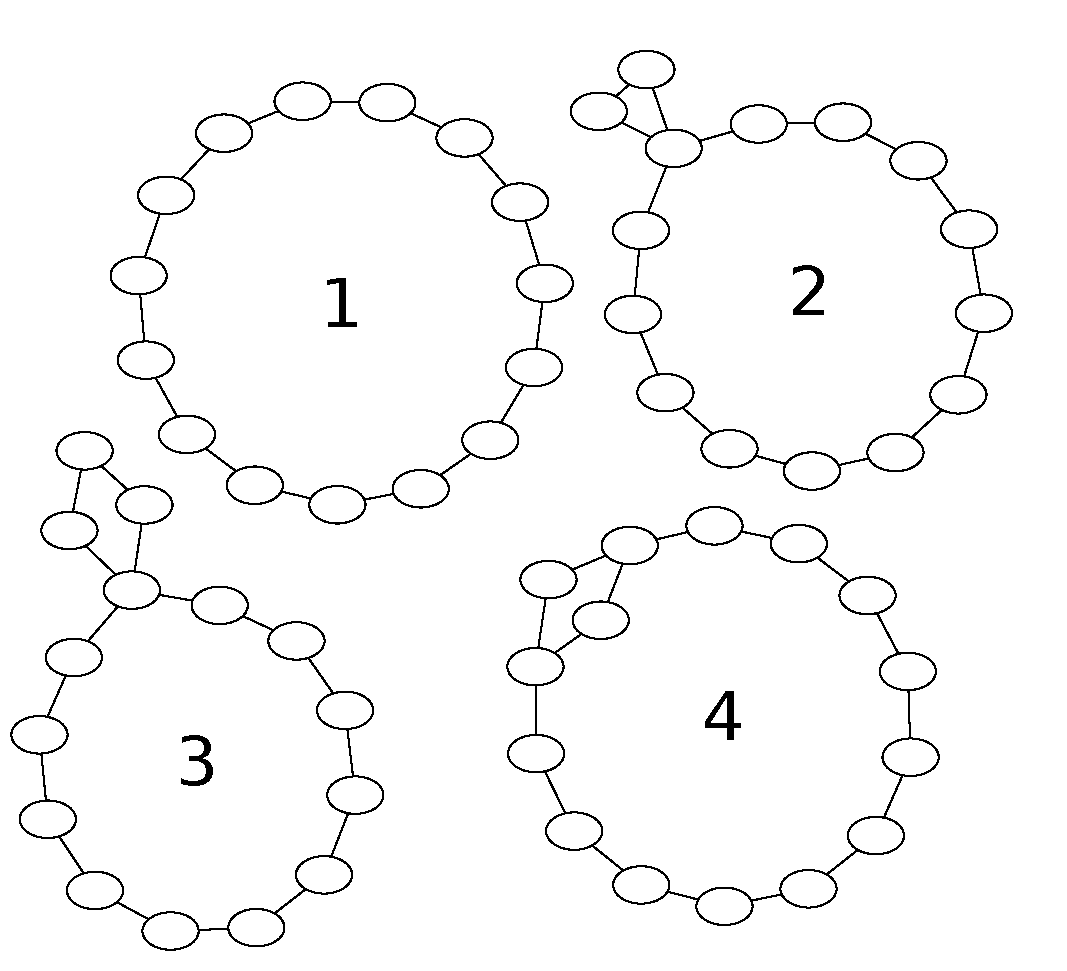
\includegraphics[width=0.9\textwidth]{images/best_ec2.pdf}}

\caption[$2$-hranovo súvislé grafy s najviac vlastnými pármi]{Ukážka štyroch pätnásťvrcholových
grafov, ktoré mali najviac vlastných párov.}

\label{graf:bestec2}
\end{figure}

